\documentclass{beamer}

\usepackage{comment}
\usepackage{color}
\usepackage{listings}
\usepackage{verbatim}
\usepackage{multicol}
\usepackage{booktabs}
\definecolor{green}{RGB}{0,128,0}

\def\EQ#1\EN{\begin{equation*}#1\end{equation*}}
\def\BA#1\EA{\begin{align*}#1\end{align*}}
\def\BS#1\ES{\begin{split*}#1\end{split*}}
\newcommand{\bc}{\begin{center}}
\newcommand{\ec}{\end{center}}
\newcommand{\eq}{\ =\ }
\newcommand{\degc}{$^\circ$C}

\def\p{\partial}
\def\qbs{\boldsymbol{q}}
\def\Dbs{\boldsymbol{D}}
\def\A{\mathcal A}
\def\gC{\mathcal C}
\def\gD{\mathcal D}
\def\gL{\mathcal L}
\def\M{\mathcal M}
\def\P{\mathcal P}
\def\Q{\mathcal Q}
\def\gR{\mathcal R}
\def\gS{\mathcal S}
\def\X{\mathcal X}
\def\bnabla{\boldsymbol{\nabla}}
\def\bnu{\boldsymbol{\nu}}
\renewcommand{\a}{{\alpha}}
%\renewcommand{\a}{{}}
\newcommand{\s}{{\sigma}}
\newcommand{\bq}{\boldsymbol{q}}
\newcommand{\bz}{\boldsymbol{z}}
\def\bPsi{\boldsymbol{\Psi}}

\def\Li{\textit{L}}
\def\Fb{\textbf{f}}
\def\Jb{\textbf{J}}
\def\cb{\textbf{c}}

\def\Dt{\Delta t}
\def\tpdt{{t + \Delta t}}
\def\bpsi{\boldsymbol{\psi}}
\def\dbpsi{\delta \boldsymbol{\psi}}
\def\bc{\textbf{c}}
\def\dbc{\delta \textbf{c}}
\def\arrows{\rightleftharpoons}

\newcommand{\bGamma}{\boldsymbol{\Gamma}}
\newcommand{\bOmega}{\boldsymbol{\Omega}}
%\newcommand{\bPsi}{\boldsymbol{\Psi}}
%\newcommand{\bpsi}{\boldsymbol{\psi}}
\newcommand{\bO}{\boldsymbol{O}}
%\newcommand{\bnu}{\boldsymbol{\nu}}
\newcommand{\bdS}{\boldsymbol{dS}}
\newcommand{\bg}{\boldsymbol{g}}
\newcommand{\bk}{\boldsymbol{k}}
%\newcommand{\bq}{\boldsymbol{q}}
\newcommand{\br}{\boldsymbol{r}}
\newcommand{\bR}{\boldsymbol{R}}
\newcommand{\bS}{\boldsymbol{S}}
\newcommand{\bu}{\boldsymbol{u}}
\newcommand{\bv}{\boldsymbol{v}}
%\newcommand{\bz}{\boldsymbol{z}}
\newcommand{\pressure}{P}

\def\water{H$_2$O}
\def\calcium{Ca$^{2+}$}
\def\copper{Cu$^{2+}$}
\def\magnesium{Mg$^{2+}$}
\def\sodium{Na$^+$}
\def\potassium{K$^+$}
\def\uranium{UO$_2^{2+}$}
\def\hion{H$^+$}
\def\hydroxide{OH$^-$}
\def\bicarbonate{HCO$_3^-$}
\def\carbonate{CO$_3^{2-}$}
\def\cotwo{CO$_2$(aq)}
\def\chloride{Cl$^-$}
\def\fluoride{F$^-$}
\def\phosphoricacid{HPO$_4^{2-}$}
\def\nitrate{NO$_3^-$}
\def\sulfate{SO$_4^{2-}$}
\def\souotwooh{$>$SOUO$_2$OH}
\def\sohuotwocothree{$>$SOHUO$_2$CO$_3$}
\def\soh{$>$SOH}

\newcommand\gehcomment[1]{{{\color{orange} #1}}}
\newcommand\add[1]{{{\color{blue} #1}}}
\newcommand\remove[1]{\sout{{\color{red} #1}}}
\newcommand\codecomment[1]{{{\color{green} #1}}}
\newcommand\redcomment[1]{{{\color{red} #1}}}
\newcommand\bluecomment[1]{{{\color{blue} #1}}}
\newcommand\greencomment[1]{{{\color{green} #1}}}
\newcommand\magentacomment[1]{{{\color{magenta} #1}}}

\begin{comment}
\tiny
\scriptsize
\footnotesize
\small
\normalsize
\large
\Large
\LARGE
\huge
\Huge
\end{comment}

\begin{document}
\title{1D Calcite Scenario\ldots in a Nutshell}
\author{Glenn Hammond}
\date{\today}

%\frame{\titlepage}

%-----------------------------------------------------------------------------
\section{Description of 1D Calcite Scenario}

\subsection{1D Calcite Conceptual Model}

\frame{\frametitle{Description of 1D Calcite Scenario}

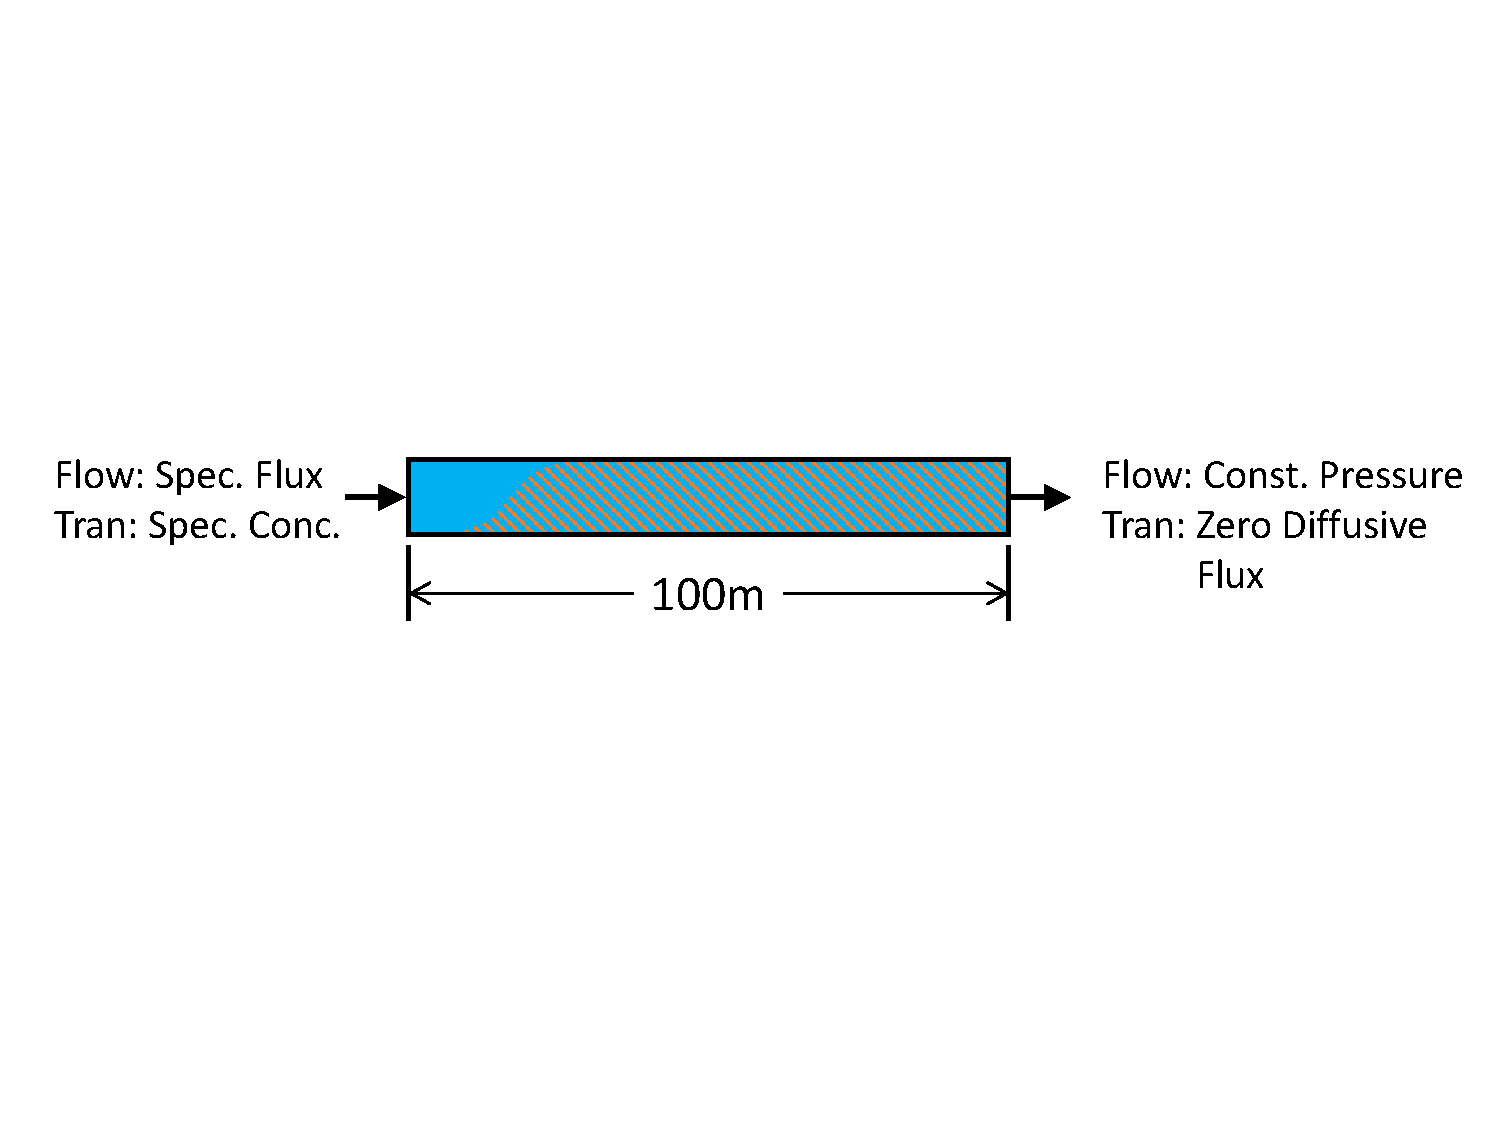
\includegraphics[width=\linewidth]{./calcite_fig}

The ``1D Calcite Scenario'' simulates solute transport along a horizontal, 1D domain measuring 100 meters in length with unit cross sectional area.  Assumptions regarding transport include:

\begin{itemize}
  \item Problem domain: $100 \times 1 \times 1$ m (x $\times$ y $\times$ z)
  \item Grid resolution $1 \times 1 \times 1$ m
  \item Darcy flow velocity: 1 m/y (left to right or west to east)
  \item Porosity: 0.25
  \item Maximum time step size: 0.25 y (CFL = 1.)
  \item Total simulation time: 25 y
\end{itemize}

}

%-----------------------------------------------------------------------------
\subsection{Governing Equations
}
\frame{\frametitle{Governing Reactive Transport Equations}

\Large

\EQ\label{trans}
\frac{\p}{\p t} \left(\varphi s \Psi_j\right) + \bnabla\cdot\bOmega_j \eq
\gR\left(c_1,c_2,\ldots,c_n\right)
\EN

\EQ\label{flux}
\bOmega_j \eq \big(\bq - \varphi s \Dbs\bnabla\big) \Psi_j
\EN

%\bigskip
%\normalsize
\footnotesize
\begin{align*}
\varphi &\eq \text{porosity}; \quad
s \eq \text{liquid saturation}\\
\Psi_j &\eq \text{total component concentration for aqueous species } j\\
c_j &\eq \text{free ion concentration for aqueous species } j\\
\bOmega &\eq \text{solute flux}; \quad
\bq \eq \text{Darcy velocity} \\
\Dbs &\eq \text{hydrodynamic dispersion} \eq\gD^\ast + \alpha_L|\bnu|\\
\gD^\ast &\eq \text{species {\color{red} independent} coefficient of diffusion}\\
\alpha_L &\eq \text{longitudinal dispersity}\\
\bnu &\eq \text{pore water velocity} \eq \bq/\varphi
\end{align*}

}

%-----------------------------------------------------------------------------
\frame{\frametitle{Reaction Equations \\{\large 1D Calcite}}

\large

\begin{align*}
\chi_i &\eq \frac{K_i}{\gamma_i} \prod_j \big(\gamma_j c_j\big)^{\nu_{ji}^{\rm aq}} \\
\Psi_j &\eq c_j + \sum_i \nu_{ji}^{\rm aq} \chi_i \eq c_j + \sum_i \nu_{ji}^{\rm aq} \frac{K_i}{\gamma_i} \prod_j \big(\gamma_j c_j\big)^{\nu_{ji}^{\rm aq}}\\
I_j &\eq -\sum_m\nu_{jm}^{\rm min} A_m k_m \left[1-K_m \prod_j \big(\gamma_j c_j\big)^{\nu_{jm}^{\rm min}}\right]
\end{align*}

%\footnotesize
\scriptsize
\begin{align*}
c_j &\eq \text{free ion concentration for aqueous species } j\\
\gamma_j &\eq \text{activity coefficient for aqueous species } j\\
\chi_i &\eq \text{secondary aqueous complex concentration } i\\
\nu_{ji} &\eq \text{stoichiometry of component $j$ in reaction } i\\
I_j &\eq \text{mineral reaction rate for species } j
\end{align*}

}

%-----------------------------------------------------------------------------
\section{Description of Input Deck: Transport Only}


%-----------------------------------------------------------------------------
\subsection{SIMULATION}

\begin{frame}[fragile]\frametitle{SIMULATION}

\begin{itemize}
  \item Specify subsurface simulation
  \item Specify the use of the transport process model
\end{itemize}


\begin{semiverbatim}

SIMULATION
  SIMULATION_TYPE SUBSURFACE
  PROCESS_MODELS
    SUBSURFACE_TRANSPORT transport \bluecomment{! process model name}
      MODE GIRT   \bluecomment{! Global Implicit Reactive Transport}
    /
  /
END

SUBSURFACE
  ...
END_SUBSURFACE
\end{semiverbatim}

\end{frame}

%-----------------------------------------------------------------------------
\subsection{GRID}
\begin{frame}[fragile,containsverbatim]\frametitle{GRID}

\begin{itemize}
  \item Problem domain: $100 \times 1 \times 1$ m (x $\times$ y $\times$ z)
  \item Grid resolution $1 \times 1 \times 1$ m
\end{itemize}

\begin{semiverbatim}
GRID
  TYPE STRUCTURED     \bluecomment{! structured grid}
  NXYZ 100 1 1        \bluecomment{! NX, NY, NZ}
  BOUNDS              \bluecomment{! define the rectangular domain}
    0.d0 0.d0 0.d0    \bluecomment{! xmin ymin zmin}
    100.d0 1.d0 1.d0  \bluecomment{! xmax ymax zmax}
  /  \bluecomment{! <-- closes out BOUNDS card}
END  \bluecomment{! <-- closes out GRID card}
\end{semiverbatim}

\end{frame}

%-----------------------------------------------------------------------------
\subsection{REGION}

\begin{frame}[fragile,containsverbatim,allowframebreaks]\frametitle{REGION}

\begin{itemize}
  \item Delineate regions in the 1D domain for:
  \begin{itemize}
    \item west boundary face
    \item east boundary face
    \item entire domain (all)
  \end{itemize}
\end{itemize}

\begin{semiverbatim}
REGION all            \bluecomment{! define a region and name it: \greencomment{all}}
  COORDINATES         \bluecomment{! using \redcomment{volumetric} coordinates}
    0.d0 0.d0 0.d0    \bluecomment{! lower coordinate: xmin ymin zmin}
    100.d0 1.d0 1.d0  \bluecomment{! upper coordinate: xmax ymax zmax}
  /   \bluecomment{! <-- closes out COORDINATES card}
END   \bluecomment{! <-- closes out REGION card}

\newpage
REGION west           \bluecomment{! define region:} \greencomment{west}
  FACE WEST           \bluecomment{! define the face of the grid cell}
  COORDINATES         \bluecomment{! using \redcomment{surface} coordinates}
    0.d0 0.d0 0.d0
    0.d0 1.d0 1.d0
  /
END

REGION east           \bluecomment{! define region:} \greencomment{east}
  FACE EAST           \redcomment{! WEST, EAST, SOUTH, NORTH,}
  COORDINATES         \redcomment{!   BOTTOM, TOP} \bluecomment{ are keywords}
    100.d0 0.d0 0.d0  \bluecomment{!   in PFLOTRAN.}
    100.d0 1.d0 1.d0
  /
END

\end{semiverbatim}

\end{frame}

%-----------------------------------------------------------------------------
\subsection{MATERIAL\_PROPERTY}

\begin{frame}[fragile,containsverbatim]\frametitle{MATERIAL\_PROPERTY}

\begin{itemize}
  \item Define a soil with :
  \begin{itemize}
    \item Material id = 1
    \item Porosity = 0.25
    \item Tortuosity = 1.
  \end{itemize}
\end{itemize}

\begin{semiverbatim}
MATERIAL_PROPERTY soil1  \bluecomment{! define a material:} \greencomment{soil1}
  ID 1                   \bluecomment{! All grid cells of this}
  POROSITY 0.25d0        \bluecomment{!   material type will have}
  TORTUOSITY 1.d0        \bluecomment{!   a material \redcomment{ID = 1}.}
END  \bluecomment{! <-- closes out MATERIAL\_PROPERTY card}
\end{semiverbatim}

\end{frame}

%-----------------------------------------------------------------------------
\subsection{FLUID\_PROPERTY}

\begin{frame}[fragile,containsverbatim]\frametitle{FLUID\_PROPERTY}

\begin{itemize}
  \item Assign a molecular diffusion coefficient of $10^{-9}$ m$^2$/s to all aqueous species
\end{itemize}

\begin{semiverbatim}

FLUID_PROPERTY                  \bluecomment{! fluid is water}
  DIFFUSION_COEFFICIENT 1.d-9   \bluecomment{! [m^2/s]}
END  \bluecomment{! <-- closes out FLUID\_PROPERTY card}
\end{semiverbatim}

\end{frame}

%-----------------------------------------------------------------------------
\subsection{CHEMISTRY}

\begin{frame}[fragile,allowframebreaks]\frametitle{CHEMISTRY}

\begin{itemize}
\item For Calcite dissolution geochemistry, specify:
  \begin{itemize}
    \item Three primary species: \hion, \bicarbonate and \calcium
    \item Six secondary aqueous complexes: \hydroxide, \carbonate, \cotwo, CaCO$_3$(aq), CaHCO$_3^+$, and CaOH$^+$
    \item One mineral: Calcite
    \item A kinetic rate for Calcite dissolution: 1.e-6 [mol/m$^2$-sec]
    \item The name of a database for species parameters (e.g. molecular weight, charge) and equilibrium constants
  \end{itemize}
\end{itemize}

\begin{semiverbatim}
CHEMISTRY
  PRIMARY_SPECIES
    H+
    HCO3-
    Ca++
  /
\end{semiverbatim}
\newpage

\begin{semiverbatim}


  SECONDARY_SPECIES
    OH-
    CO3--
    CO2(aq)
    CaCO3(aq)
    CaHCO3+
    CaOH+
  /
  PASSIVE_GAS_SPECIES
    CO2(g)
  /
\end{semiverbatim}
\newpage

\begin{semiverbatim}


  MINERALS
    Calcite
  /
  MINERAL_KINETICS
    Calcite       \bluecomment{! Note: mineral name opens block}
      RATE_CONSTANT 1.d-6 mol/m^2-sec
    /
  /
\end{semiverbatim}
\newpage

\begin{semiverbatim}


  DATABASE ../../../hanford.dat  \bluecomment{! path to database file}
  LOG_FORMULATION         \bluecomment{! logarithmic derivatives}
  ACTIVITY_COEFFICIENTS TIMESTEP  \bluecomment{! time step lagged}
  OUTPUT                          \bluecomment{!   activity}
    PH                            \bluecomment{!   coefficients}
    TOTAL     \bluecomment{! total component concentrations}
    ALL       \bluecomment{! print primary species}
  /
END

\end{semiverbatim}

\end{frame}

%-----------------------------------------------------------------------------
\subsection{CONSTRAINT}

\begin{frame}[fragile,allowframebreaks]\frametitle{CONSTRAINT}

\begin{itemize}
  \item Set up solute concentrations and geochemical constraints
\end{itemize}

\begin{semiverbatim}

CONSTRAINT initial_constraint \bluecomment{! named: \greencomment{initial_constraint}}
  CONCENTRATIONS           \bluecomment{! concentration block}
    H+     1.d-8      F    \bluecomment{! \redcomment{F} = free ion}
    HCO3-  1.d-3      G  CO2(g) \bluecomment{! \redcomment{G} = equil. w/ gas [bar]}
    Ca++   5.d-4      M  Calcite \bluecomment{! \redcomment{M} = equil. w/ mineral}
  /  \bluecomment{    ! ^^^^^ \redcomment{5.e-4} is a guess}
  MINERALS               \bluecomment{! mineral block}
            \bluecomment{! vol. frac. = \redcomment{1.e-5}; area = \redcomment{1.}}
    Calcite 1.d-5 1.d0 m^2/m^3
  /  \bluecomment{! <-- closes out MINERAL block}
END  \bluecomment{! <-- closes out CONSTRAINT card}

\newpage
CONSTRAINT inlet_constraint \bluecomment{! named: \greencomment{inlet_constraint}}
  CONCENTRATIONS
    H+     5.         P  \bluecomment{! \redcomment{P} = pH; analogous to -log(F)}
    HCO3-  1.d-3      T  \bluecomment{! \redcomment{T} = total component}
    Ca++   1.d-6      Z  \bluecomment{! \redcomment{Z} = charge balance}
  /  \bluecomment{! <-- closes out block; \redcomment{note no MINERAL block}}
END

\end{semiverbatim}

\end{frame}

%-----------------------------------------------------------------------------
\subsection{TRANSPORT\_CONDITION}

\begin{frame}[fragile,allowframebreaks]\frametitle{TRANSPORT\_CONDITION}

\begin{itemize}
  \item Couple transport constraints with transport conditions
\end{itemize}
\begin{semiverbatim}
TRANSPORT_CONDITION background_conc \bluecomment{! named \greencomment{background...}}
  TYPE ZERO_GRADIENT       \bluecomment{! this is a \redcomment{zero gradient} bc}
  CONSTRAINT_LIST          \bluecomment{! list of constraints}
    \bluecomment{! start constraint \redcomment{initial_constraint} @ time = \redcomment{0.}}
    0.d0 initial_constraint
  /  \bluecomment{! <-- closes out CONSTRAINT\_LIST block}
END  \bluecomment{! <-- closes out TRANSPORT\_CONDITION block}

TRANSPORT_CONDITION inlet_conc  \bluecomment{! named \greencomment{inlet_conc}}
  TYPE DIRICHLET_ZERO_GRADIENT  \bluecomment{! \redcomment{dirichlet_zero_gradient}}
  CONSTRAINT_LIST               \bluecomment{! inflow = Dirichlet}
    0.d0 inlet_constraint       \bluecomment{! outflow = zero grad.}
  /    \bluecomment{! ^^^^^ constraint and transport condition}
END    \bluecomment{!         names need not match}

\end{semiverbatim}

\end{frame}

%-----------------------------------------------------------------------------
\subsection{STRATA}

\begin{frame}[fragile]\frametitle{STRATA}

\begin{itemize}
\item Couple \greencomment{soil1} rock/soil type with region \greencomment{all} to define a stratigraphic unit
\end{itemize}

\begin{semiverbatim}

STRATA
  REGION all
  MATERIAL soil1
END


\end{semiverbatim}

\end{frame}

%-----------------------------------------------------------------------------
\subsection{INITIAL\_CONDITION}

\begin{frame}[fragile]\frametitle{INITIAL\_CONDITION}

\begin{itemize}
\item Couple the \greencomment{initial} transport condition with region \greencomment{all} for the initial condition
\end{itemize}

\begin{semiverbatim}

INITIAL_CONDITION               \bluecomment{! notice no name}
  TRANSPORT_CONDITION background_conc
  REGION all
END

\end{semiverbatim}

\end{frame}

%-----------------------------------------------------------------------------
\subsection{BOUNDARY\_CONDITION}

\begin{frame}[fragile]\frametitle{BOUNDARY\_CONDITION}

\begin{itemize}
\item Couple the \greencomment{inlet\_conc} transport condition with region \greencomment{west} for the \redcomment{inlet} boundary condition.
\item Couple the \greencomment{background\_conc} transport condition with region \greencomment{east} for the \redcomment{outlet} boundary condition.
\end{itemize}

\begin{semiverbatim}

BOUNDARY_CONDITION outlet             \bluecomment{! name is optional,}
  TRANSPORT_CONDITION background_conc \bluecomment{!   but recommended}
  REGION east
END

BOUNDARY_CONDITION inlet
  TRANSPORT_CONDITION inlet_conc
  REGION west
END

\end{semiverbatim}

\end{frame}

%-----------------------------------------------------------------------------
\subsection{LINEAR\_SOLVER}

\begin{frame}[fragile]\frametitle{LINEAR\_SOLVER}

\begin{itemize}
\item Due to the small problem size, request a direct solver.
\item PETSc provides a direct solve through LU matrix factorization as a preconditioner with no outer Krylov solve.
\end{itemize}

\begin{semiverbatim}

NUMERICAL_METHODS TRANSPORT
  LINEAR_SOLVER           \bluecomment{! transport solver}
    SOLVER DIRECT         \bluecomment{! sets both the below}
  /
END

  \bluecomment{! could also use:}
  LINEAR_SOLVER
    KSP_TYPE PREONLY        \bluecomment{! turn off Krylov solver}
    PC_TYPE PCLU            \bluecomment{! LU preconditioner}
  /

\end{semiverbatim}

\end{frame}

%-----------------------------------------------------------------------------
\subsection{TIME}

\begin{frame}[fragile]\frametitle{TIME}

\begin{itemize}
\item Set final simulation time to 25 years
\item Set initial time step size to 1. h
\item Set maximum time step size to 0.25 years
\end{itemize}


\begin{semiverbatim}

TIME
  FINAL_TIME 25.d0 \redcomment{y}            \bluecomment{! Within TIME, time units}
  INITIAL_TIMESTEP_SIZE 1.d0 \redcomment{h}    \bluecomment{! are recognized and}
  MAXIMUM_TIMESTEP_SIZE 2.5d-1 \redcomment{y}  \bluecomment{! converted to SI}
END                               \bluecomment{! (i.e. \redcomment{y}, \redcomment{h} --> \greencomment{s}).}
\end{semiverbatim}

\end{frame}

%-----------------------------------------------------------------------------
\subsection{OUTPUT}

\begin{frame}[fragile]\frametitle{OUTPUT}

\begin{itemize}
\item Specify output times (5, 10, 15, 20 years) and format (Tecplot point datapacking).
\item The initial and final simulation times are automatically added to the list of output times.
\item Note that additional output options (e.g. species names) are specified within CHEMISTRY.
\end{itemize}


\begin{semiverbatim}

OUTPUT
  TIMES \redcomment{y} 5. 10. 15. 20.  \bluecomment{! Within OUTPUT, time units}
  FORMAT TECPLOT POINT    \bluecomment{! are recognized and}
END                       \bluecomment{! converted to SI}
                          \bluecomment{! (i.e. \redcomment{y} --> \greencomment{s}).}
\end{semiverbatim}

\end{frame}

%-----------------------------------------------------------------------------
\subsection{Miscellaneous}

\begin{frame}[fragile]\frametitle{Miscellaneous}

\begin{itemize}
\item Specify a uniform Darcy velocity of 1 m/y in x-direction
\end{itemize}


\begin{semiverbatim}

SPECIFIED_VELOCITY
  UNIFORM? YES
  DATASET 1.d0 0.d0 0.d0 m/yr
END
\end{semiverbatim}

\end{frame}

%-----------------------------------------------------------------------------
\subsection{Running calcite_tran_only.in}

\begin{frame}[fragile]\frametitle{Running PFLOTRAN}

\begin{semiverbatim}

> cd $PFLOTRAN_DIR
> cd shortcourse/exercises/1D_Calcite
> pflotran -input_prefix calcite_tran_only
> python conc_at_25y_tran_only.py
> python pH_tran_only.py

\end{semiverbatim}

\end{frame}

%-----------------------------------------------------------------------------
\section{Description of Input Deck: Adding a flow solution}

\subsection{Input File Modifications}

\begin{frame}[fragile]\frametitle{Adding a flow solution}

Input File Modifications
\begin{itemize}
\item Modify cards:
  \begin{itemize}
    \item SIMULATION
    \item MATERIAL\_PROPERTY
    \item INITIAL\_CONDITION
    \item BOUNDARY\_CONDITION
   \end{itemize}
\item Add cards:
  \begin{itemize}
    \item LINEAR\_SOLVER (for flow)
    \item CHARACTERISTIC\_CURVES
    \item FLOW\_CONDITION
  \end{itemize}
\item Remove cards:
  \begin{itemize}
    \item SPECIFIED\_VELOCITY
  \end{itemize}
\end{itemize}

\end{frame}

%-----------------------------------------------------------------------------
\subsection{SIMULATION}

\begin{frame}[fragile]\frametitle{SIMULATION}

\begin{itemize}
  \item Add flow process model
\end{itemize}


\begin{semiverbatim}
SIMULATION
  SIMULATION_TYPE SUBSURFACE
  PROCESS_MODELS
    \magentacomment{SUBSURFACE_FLOW flow}  \bluecomment{! flow process model}
      \magentacomment{MODE RICHARDS}       \bluecomment{! single phase variably-}
    \magentacomment{/}                     \bluecomment{!   saturated flow}
    SUBSURFACE_TRANSPORT transport
      MODE GIRT
    /
  /
END

SUBSURFACE
  ...
END_SUBSURFACE
\end{semiverbatim}

\end{frame}

%-----------------------------------------------------------------------------
\subsection{MATERIAL\_PROPERTY}

\begin{frame}[fragile]\frametitle{MATERIAL\_PROPERTY}

\begin{itemize}
\item Add isotropic permeability of 1 Darcy (1.e-12 m$^2$)
\end{itemize}

\begin{semiverbatim}
MATERIAL_PROPERTY soil1
  ID 1
  POROSITY 0.25d0
  TORTUOSITY 1.d0
  \magentacomment{PERMEABILITY}     \bluecomment{! permeability is defined in a block}
    \magentacomment{PERM_ISO 1.d-12}  \bluecomment{! isotropic permeability}
  \magentacomment{/}
  \magentacomment{CHARACTERISTIC_CURVES default}  \bluecomment{! couple the saturation}
END                              \bluecomment{!   function}
\end{semiverbatim}

\end{frame}

%-----------------------------------------------------------------------------
\subsection{INITIAL\_CONDITION}

\begin{frame}[fragile]\frametitle{INITIAL\_CONDITION}

\begin{itemize}
\item Add the \greencomment{initial} flow condition
\end{itemize}

\begin{semiverbatim}

INITIAL_CONDITION              \bluecomment{! flow and transport}
  \magentacomment{FLOW_CONDITION initial_pressure}
  TRANSPORT_CONDITION background_conc
  REGION all
END

\end{semiverbatim}

\end{frame}

%-----------------------------------------------------------------------------
\subsection{BOUNDARY\_CONDITION}

\begin{frame}[fragile]\frametitle{BOUNDARY\_CONDITION}

\begin{itemize}
\item Add the \greencomment{inlet\_flux} flow condition to the \redcomment{inlet} boundary condition.
\item Add the \greencomment{initial\_pressure} flow condition to the \redcomment{outlet} boundary condition.
\end{itemize}

\begin{semiverbatim}

BOUNDARY_CONDITION outlet
  \magentacomment{FLOW_CONDITION initial_pressure}
  TRANSPORT_CONDITION background_conc
  REGION east
END

BOUNDARY_CONDITION inlet
  \magentacomment{FLOW_CONDITION inlet_flux}
  TRANSPORT_CONDITION inlet_conc
  REGION west
END

\end{semiverbatim}

\end{frame}

%-----------------------------------------------------------------------------
\subsection{LINEAR\_SOLVER}

\begin{frame}[fragile]\frametitle{LINEAR\_SOLVER}

\begin{itemize}
\item As with transport, use the direct solver for this small problem.
\end{itemize}


\begin{semiverbatim}

\magentacomment{NUMERICAL_METHODS FLOW}
  \magentacomment{LINEAR_SOLVER}
    \magentacomment{SOLVER DIRECT}
  \magentacomment{/}
\magentacomment{END}

\bluecomment{! the original transport solver}
NUMERICAL_METHODS TRANSPORT
  LINEAR_SOLVER TRANSPORT 
    SOLVER DIRECT
  /
END
\end{semiverbatim}

\end{frame}

%-----------------------------------------------------------------------------
\subsection{CHARACTERISTIC\_CURVES}

\begin{frame}[fragile]\frametitle{CHARACTERISTIC\_CURVES}

\begin{itemize}
\item Assume saturated flow
\item Add default (dummy) characteristic curves
\item For variably-saturated flow, one would include parameters such as the air entry pressure, residual saturation, van Genuchten ``n'', etc. in the characteristic curves definition, \gehcomment{but ignore this for now}.
\end{itemize}

\begin{semiverbatim}

\magentacomment{CHARACTERISTIC_CURVES default
  DEFAULT
END}
\end{semiverbatim}

\end{frame}

%-----------------------------------------------------------------------------
\subsection{FLOW\_CONDITION}

\begin{frame}[fragile]\frametitle{FLOW\_CONDITION}

\begin{itemize}
\item Specify an initial pressure
\item Specify a boundary flux at inlet
\end{itemize}

\begin{semiverbatim}
\magentacomment{FLOW_CONDITION initial_pressure} \bluecomment{! named \greencomment{initial_pressure}}
  \magentacomment{TYPE
    LIQUID_PRESSURE DIRICHLET} \bluecomment{! type is \redcomment{dirichlet} for}
  \magentacomment{/}                           \bluecomment{!   constant pressure [Pa]}
  \magentacomment{LIQUID_PRESSURE 201325.d0}   \bluecomment{! greater than atmospheric}
\magentacomment{END}                           \bluecomment{!   to ensure saturation}

\magentacomment{FLOW_CONDITION inlet_flux} \bluecomment{! named \greencomment{inlet_flux}}
  \magentacomment{TYPE
    LIQUID_FLUX NEUMANN}    \bluecomment{! type is \redcomment{neumann} for a flux}
  \magentacomment{/
  LIQUID_FLUX 1.d0 m/yr}    \bluecomment{! Darcy velocity of 1 m/y}
\magentacomment{END}
\end{semiverbatim}

\end{frame}

%-----------------------------------------------------------------------------
\subsection{Running calcite_flow_and_tran.in}

\begin{frame}[fragile]\frametitle{Running PFLOTRAN}

\begin{semiverbatim}

> cd $PFLOTRAN_DIR
> cd shortcourse/exercises/1D_Calcite
> pflotran -input_prefix calcite_flow_and_tran
> python conc_at_25y_flow_and_tran.py
> python pH_flow_and_tran.py
\end{semiverbatim}

\end{frame}

%-----------------------------------------------------------------------------
\section{Description of Input Deck: Switch to infiltration}

\subsection{Input File Modifications}

\begin{frame}[fragile]\frametitle{Switch to Infiltration: Calcite Leaching}

Input File Modifications
\begin{itemize}
%\item Add cards:
%  \begin{itemize}
%    \item
%  \end{itemize}
\item Modify cards:
  \begin{itemize}
    \item GRID
    \item MATERIAL\_PROPERTY
    \item CHARACTERISTIC\_CURVES
    \item FLOW\_CONDITION
    \item BOUNDARY\_CONDITION
   \end{itemize}
\end{itemize}

\end{frame}

%-----------------------------------------------------------------------------
\subsection{GRID}
\begin{frame}[fragile,containsverbatim]\frametitle{GRID}

\begin{itemize}
  \item Problem domain: $1 \times 1 \times 10$ m (x $\times$ y $\times$ z)
  \item Grid resolution $1 \times 1 \times 0.1$ m
\end{itemize}

\begin{semiverbatim}
GRID
  TYPE STRUCTURED
  NXYZ \magentacomment{1} 1 \magentacomment{100}     \bluecomment{! Switch to Z}
  BOUNDS
    0.d0 0.d0 0.d0
    \magentacomment{1.d0} 1.d0 \magentacomment{10.d0}  \bluecomment{! 1 m in X, 10 m in Z}
  /
END
\end{semiverbatim}

\end{frame}

%-----------------------------------------------------------------------------
\subsection{MATERIAL\_PROPERTY}

\begin{frame}[fragile]\frametitle{MATERIAL\_PROPERTY}

\begin{itemize}
\item Change name of saturation function
\end{itemize}

\begin{semiverbatim}
MATERIAL_PROPERTY soil1
  ID 1
  POROSITY 0.25d0
  TORTUOSITY 1.d0
  PERMEABILITY
    PERM_ISO 1.d-12
  /
  CHARACTERISTIC\_CURVES \magentacomment{cc1}
END
\end{semiverbatim}

\end{frame}

%-----------------------------------------------------------------------------
\subsection{CHARACTERISTIC\_CURVES}

\begin{frame}[fragile]\frametitle{CHARACTERISTIC\_CURVES}

\begin{itemize}
\item Add van Genuchten saturation function parameters
\item Assume Mualem relative permeability (default)
\end{itemize}

\begin{semiverbatim}
CHARACTERISTIC_CURVES \magentacomment{cc1
  SATURATION_FUNCTION VAN_GENUCHTEN
    ALPHA  1.d-4}    \bluecomment{! [Pa^-1]}
    \magentacomment{M 0.5d0}         \bluecomment{! van Genuchten m in n = 1/(1-m)}
    \magentacomment{LIQUID_RESIDUAL_SATURATION 0.1d0
    MAX_CAPILLARY_PRESSURE 1.d8
  /
  PERMEABILITY_FUNCTION MUALEM_VG_LIQ
    M 0.5d0
    LIQUID_RESIDUAL_SATURATION 0.1d0
  /}
END
\end{semiverbatim}

\end{frame}

%-----------------------------------------------------------------------------
\subsection{REGION}

\begin{frame}[fragile,containsverbatim,allowframebreaks]\frametitle{REGION}

\begin{itemize}
  \item Change coordinates for new domain
  \item Change faces for top and bottom, instead of west/east
\end{itemize}

\begin{semiverbatim}

REGION all
  COORDINATES
    0.d0 0.d0 0.d0
    \magentacomment{1.d0} 1.d0 \magentacomment{10.d0}
  /
END

\newpage\magentacomment{REGION top
  FACE TOP
  COORDINATES
    0.d0 0.d0 10.d0
    1.d0 1.d0 10.d0
  /
END}

\magentacomment{REGION bottom
  FACE BOTTOM
  COORDINATES
    0.d0 0.d0 0.d0
    1.d0 1.d0 0.d0
  /
END}

\end{semiverbatim}

\end{frame}

%-----------------------------------------------------------------------------
\subsection{FLOW\_CONDITION}

\begin{frame}[fragile]\frametitle{FLOW\_CONDITION}

\begin{itemize}
\item Change initial condition to type hydrostatic
\item Specify the datum for the water table
\item Modify Darcy flux to reflect recharge
\end{itemize}

\begin{semiverbatim}
FLOW_CONDITION initial_pressure
  TYPE
    LIQUID_PRESSURE \magentacomment{HYDROSTATIC} \bluecomment{! pressure as a function}
  /                             \bluecomment{!   of elevation}
  \magentacomment{DATUM 0.d0 0.d0 1.d0}          \bluecomment{! location of water table}
  LIQUID_PRESSURE \magentacomment{101325.d0}     \bluecomment{! atmospheric pressure}
END

FLOW_CONDITION \magentacomment{recharge}
  TYPE
    LIQUID_FLUX NEUMANN
  /
  LIQUID_FLUX \magentacomment{10 cm/y}           \bluecomment{! Darcy velocity}
END

\end{semiverbatim}

\end{frame}

%-----------------------------------------------------------------------------
\subsection{BOUNDARY\_CONDITION}

\begin{frame}[fragile]\frametitle{BOUNDARY\_CONDITION}

\begin{itemize}
\item Change names of regions
\item Change name of flow condition in \redcomment{inlet} boundary condition to \greencomment{recharge}
\end{itemize}

\begin{semiverbatim}

BOUNDARY_CONDITION outlet
  FLOW_CONDITION initial_pressure
  TRANSPORT_CONDITION background_conc
  REGION \magentacomment{bottom}
END

BOUNDARY_CONDITION inlet
  FLOW_CONDITION \magentacomment{recharge}
  TRANSPORT_CONDITION inlet_conc
  REGION \magentacomment{top}
END
\end{semiverbatim}

\end{frame}


%-----------------------------------------------------------------------------
\subsection{Running calcite_vsat_flow_and_tran.in}

\begin{frame}[fragile]\frametitle{Running PFLOTRAN}

\begin{semiverbatim}

> cd $PFLOTRAN_DIR
> cd shortcourse/exercises/1D_Calcite
> pflotran -input_prefix calcite_vsat_flow_and_tran
> python pH_vsat.py
\end{semiverbatim}

\end{frame}

\end{document}
